%Salto de pagina
%\pagebreak

\section{Cronograma de actividades}

\begin{table}[ht]
\centering
\begin{tabular}{|c|l|c|c|c|}
\hline
  & Nombre de tareas & Duración (Dias) & Comienzo & Fin\tabularnewline
\hline
\hline
1 & Escritura Manuscrito (Tesis) & 478 & 01/02/2017 & 30/11/2018
\tabularnewline
\hline
2 & Examen de Grado & 6 & 03/12/2018 & 10/12/2018
\tabularnewline
\hline
3 & Asistencia a Congreso 2017 & 21 & 01/09/2017 & 29/09/2017
\tabularnewline
\hline
4 & Publicación Articulo & 22 & 01/03/2018 & 30/03/2018
\tabularnewline
\hline
5 & Asistencia a Congreso 2018 & 20 & 03/09/2018 & 28/09/2018
\tabularnewline
\hline
6 & Diseño de la propuesta & 23 & 01/08/2017 & 31/08/2017
\tabularnewline
\hline
7 & Programar el Recolector de Datos & 23 & 01/08/2017 & 31/08/2017
\tabularnewline
\hline
8 & Desarrollo del Software & 66 & 01/09/2017 & 01/12/2017
\tabularnewline
\hline
9 & Pruebas del Software & 66 & 04/12/2017 & 05/03/2018
\tabularnewline
\hline
10 & Recolectar Datos de Prueba & 129 & 01/09/2017 & 28/02/2018
\tabularnewline
\hline
\end{tabular}
\caption{Cronograma de Actividades.}
\end{table}


\begin{figure}[h]
\centering
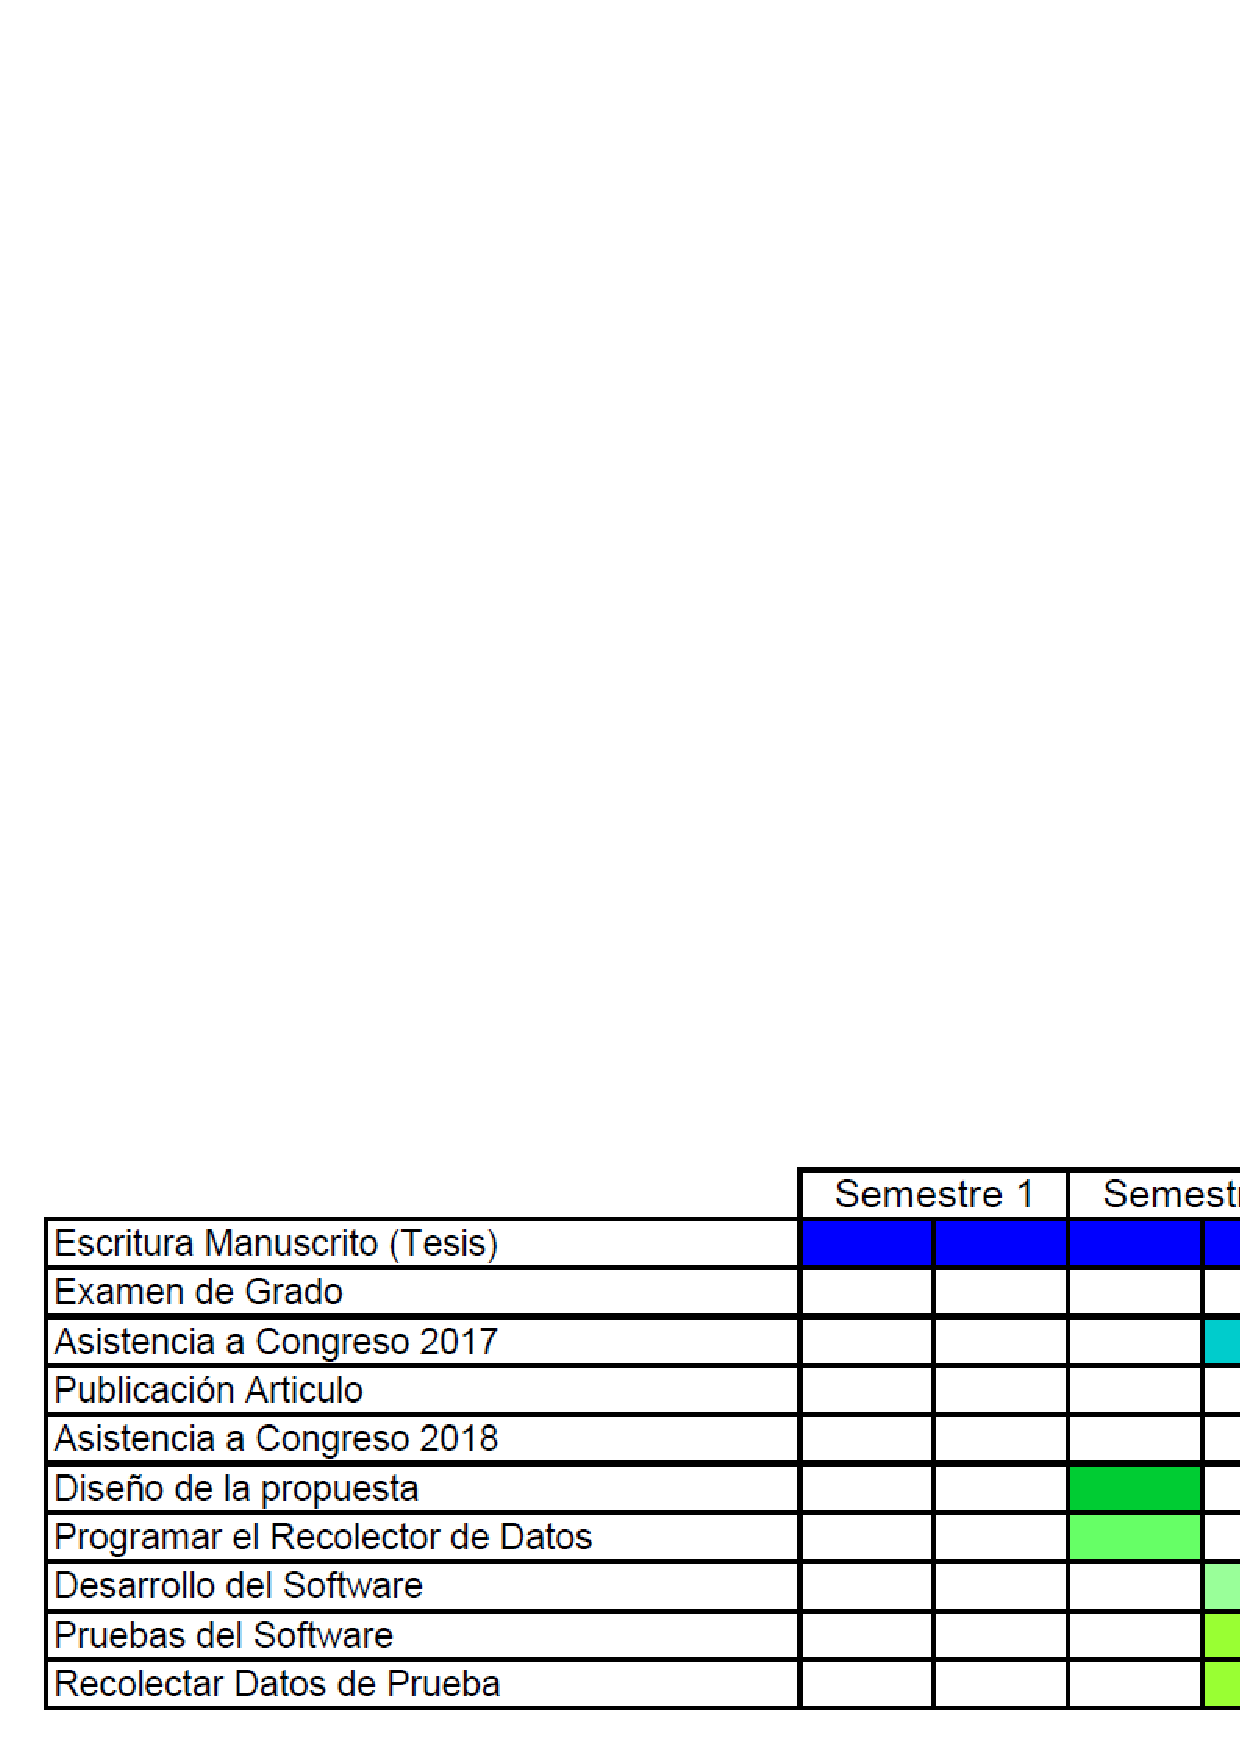
\includegraphics[width=1.0\columnwidth]{./CapituloI/Imagenes/Cronograma.PNG}
\caption{Gráfica de GANTT del cronograma de actividades.}
\end{figure}